
The four color theorem was initially formulated from a problem in coloring world maps. A map consists of regions that can border other regions on a flat surface. When we talk about a \textit{coloring} of a map, we mean a way to color its regions such that any two neighbors are colored differently.

The actual shape of the regions in our map is not of importance here. The key information that is needed from a map, is the connectivity between regions. Such information can be represented in a \textit{graph} where vertices (circles) correspond to regions. An edge between two vertices then indicates that the two corresponding regions are neighbors.

\begin{figure}[!h]
    \centering
    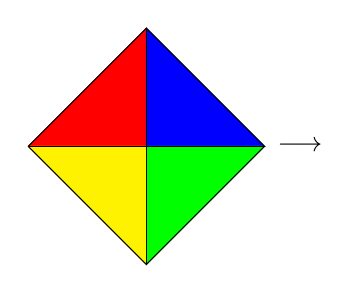
\begin{tikzpicture}[scale=1.5]
        \coordinate (v1) at (-1, 0);
        \coordinate (v2) at (0, 1);
        \coordinate (v3) at (1, 0);
        \coordinate (v4) at (0, -1);
        \coordinate (c) at (0, 0);

        \draw [fill, red] (v1) -- (v2) -- (c) -- (v1);
        \draw [fill, blue] (v2) -- (v3) -- (c) -- (v2);
        \draw [fill, green] (v3) -- (v4) -- (c) -- (v3);
        \draw [fill, yellow] (v4) -- (v1) -- (c) -- (v4);
        \draw (v1) -- (v2) -- (v3) -- (v4) -- (v1);
        \draw (c) -- (v1);
        \draw (c) -- (v2);
        \draw (c) -- (v3);
        \draw (c) -- (v4);
        \node at (1.3, 0) { $\longrightarrow$ };
    \end{tikzpicture} 
    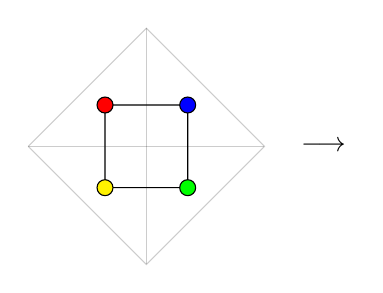
\begin{tikzpicture}[scale=1.5]
        \coordinate (v1) at (-1, 0);
        \coordinate (v2) at (0, 1);
        \coordinate (v3) at (1, 0);
        \coordinate (v4) at (0, -1);
        \coordinate (c) at (0, 0);

        \node[circle, fill, scale=0.01cm, red, draw=black] (m1) at (-0.35, 0.35) { $v_1$ };
        \node[circle, fill, scale=0.01cm, blue, draw=black] (m2) at (0.35, 0.35) { $v_2$ };
        \node[circle, fill, scale=0.01cm, green, draw=black] (m3) at (0.35, -0.35) { $v_3$ };
        \node[circle, fill, scale=0.01cm, yellow, draw=black] (m4) at (-0.35, -0.35) { $v_4$ };

        \draw (m1) -- (m2) -- (m3) -- (m4) -- (m1);
        \draw[opacity=0.2] (v1) -- (v2) -- (v3) -- (v4) -- (v1);
        \draw[opacity=0.2] (c) -- (v1);
        \draw[opacity=0.2] (c) -- (v2);
        \draw[opacity=0.2] (c) -- (v3);
        \draw[opacity=0.2] (c) -- (v4);
        \node at (1.5, 0) { $\longrightarrow$ };
    \end{tikzpicture}  
    \begin{tikzpicture}[scale=1.5, mid arrow/.style={
        postaction={ decorate, decoration={ markings, mark=at position 0.6 with { \arrow[black]{>>} } } } }]
        \coordinate (v1) at (-1, 0);
        \coordinate (v2) at (0, 1);
        \coordinate (v3) at (1, 0);
        \coordinate (v4) at (0, -1);
        \coordinate (c) at (0, 0);

        \node[circle, fill, scale=0.015cm, label=above left:$a$] (m1) at (-0.35, 0.35) { };
        \node[circle, fill, scale=0.015cm, label=above right:$b$] (m2) at (0.35, 0.35) { };
        \node[circle, fill, scale=0.015cm, label=below right:$c$] (m3) at (0.35, -0.35) { };
        \node[circle, fill, scale=0.015cm, label=below left:$d$] (m4) at (-0.35, -0.35) { };

        \draw[mid arrow] (m1) -- (m2);
        \draw (m2) -- (m3) -- (m4) -- (m1);
        \draw[opacity=0.0] (v1) -- (v2) -- (v3) -- (v4) -- (v1);
    \end{tikzpicture}      
    \caption{The translation of a map coloring to a graph coloring. In the last step we replace colors by the letters $a$,$b$,$c$ and $d$ for convenience. We obtain the coloring called $abcd$ on a \textit{planar graph}. }
    \label{fig:colortut}
\end{figure}

We will be working exclusively with \textit{planar graphs}. See Figure \ref{fig:planartut} for examples. The order of colors such as in $abcd$ is indicated by the $\gg$ edge, which is the first edge between the first two vertices. Two colorings are considered \textit{equal} if they differ only by a renaming of colors.

\begin{definition}
    A graph is \emph{planar} if it has a \emph{planar embedding} where no two edges cross each other.
\end{definition}
\begin{definition}
    \label{def:coleq}
    Two colorings $x$ and $y$ are \emph{equal} if they differ only by a renaming of the colors $a,b,c$ and $d$. I.e $abab = acac$.
\end{definition}

\begin{theorem}
    Every planar graph can be colored in at most four colors.
\end{theorem}

\begin{figure}
    \centering
    \begin{tikzpicture}[scale=1.5]
        \coordinate (v1) at (-1, 0);
        \coordinate (v2) at (0, 1);
        \coordinate (v3) at (1, 0);
        \coordinate (v4) at (0, -1);
        \coordinate (c) at (0, 0);

        \node[circle, fill, scale=0.015cm] (m1) at (-0.35, 0.35) { };
        \node[circle, fill, scale=0.015cm] (m2) at (0.35, 0.35) { };
        \node[circle, fill, scale=0.015cm] (m3) at (0.35, -0.35) { };
        \node[circle, fill, scale=0.015cm] (m4) at (-0.35, -0.35) { };

        \draw (m1) -- (m2);
        \draw (m2) -- (m3) -- (m4) -- (m1);
        \draw (m1) -- (m3);
        \draw (m2) -- (m4);
        \draw[opacity=0.0] (v1) -- (v2) -- (v3) -- (v4) -- (v1);
    \end{tikzpicture}
    \begin{tikzpicture}[scale=1.5]
        \coordinate (v1) at (-1, 0);
        \coordinate (v2) at (0, 1);
        \coordinate (v3) at (1, 0);
        \coordinate (v4) at (0, -1);
        \coordinate (c) at (0, 0);

        \node[circle, fill, scale=0.015cm] (m1) at (-0.35, 0.35) { };
        \node[circle, fill, scale=0.015cm] (m2) at (0.35, 0.35) { };
        \node[circle, fill, scale=0.015cm] (m3) at (0.35, -0.35) { };
        \node[circle, fill, scale=0.015cm] (m4) at (-0.35, -0.35) { };

        \draw (m2) -- (m4);
        \draw (m1) .. controls +(0.7, 0.7) and +(0.7, 0.7) .. (m3);
        \draw (m1) -- (m2);
        \draw (m2) -- (m3) -- (m4) -- (m1);
        \draw[opacity=0.0] (v1) -- (v2) -- (v3) -- (v4) -- (v1);
    \end{tikzpicture}
    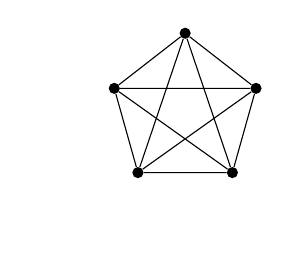
\begin{tikzpicture}
        \node[circle, fill, scale=0.015cm] (l1) at (0, 1) { };
        \node[circle, fill, scale=0.015cm] (l2) at (0.9, 0.30) { };
        \node[circle, fill, scale=0.015cm] (l3) at (0.6, -0.77) {};
        \node[circle, fill, scale=0.015cm] (l4) at (-0.6, -0.77) {};
        \node[circle, fill, scale=0.015cm] (l5) at (-0.9, 0.30) {};
        \node[circle, fill, scale=0cm] at (-2, -1.5) {};

        \draw (l1) -- (l3) -- (l5) -- (l2) -- (l4) -- (l1);
        \draw (l1) -- (l2) -- (l3) -- (l4) -- (l5) -- (l1);
        
    \end{tikzpicture}
    \caption{A non-planar embedding of the full graph $K_4$ on 4 vertices (left). A planar embedding of $K_4$ (middle), therefore $K_4$ is a planar graph. A non-planar graph $K_5$ that has no planar embeddings (right). }
    \label{fig:planartut}
\end{figure}